\documentclass[11pt]{article}
\usepackage[margin=0.85in]{geometry}
\usepackage{booktabs,graphicx,amsmath,hyperref,caption,float}
\title{Phase 2: Descriptive Probability Analysis of MoCA and Entorhinal Volume}
\author{Statistics Project -- NACC UDS + MRI subset}
\date{}
\begin{document}\maketitle
\begin{abstract}This report describes empirical probabilities and distributions among supplied, linked participants aged 65 years or older. It examines dataset-coded cognitive status and bilateral entorhinal volume. The analysis is descriptive and does not estimate general-population prevalence or causal effects.\end{abstract}
\section{Research question and Phase 1 continuity}
Among unique participants aged at least 65 in the supplied linked NACC UDS and MRI subset, how do empirical probabilities of MCI or dementia vary across groups defined by bilateral entorhinal volume, and what are the distributions and linear association of MoCA score and volume? Phase 1's conventions are retained: NACCID as participant key; NACCAGE $\geq65$; MOCATOTS valid only in [0,30], without rounding or clipping; EDUC=99 unknown; and bilateral MRI measurement as the arithmetic mean of valid positive left and right values. NACCUDSD is coded 1=Normal, 2=Impaired not MCI, 3=MCI, and 4=Dementia.
\section{Data, unit, linkage, and limits}
Each CSV contains a single supplied row per unique NACCID. The script verifies uniqueness and agreement of NACCUDSD across files, links by ID, then applies the age rule. The main analysis retains this one record per participant. The files lack visit identifiers/dates and MRI scan dates; therefore this record cannot be established as a baseline, nor can contemporaneous UDS--MRI measurement be established. The UDS file is processed/imputed, but the imputation procedure and original missingness mask are unavailable; no blank cells do not prove that original observations were complete. The supplied subset is a clinical/research subset, not a probability sample of older adults generally.
\begin{table}[H]\centering\caption{Analytic flow and valid sample sizes}\begin{tabular}{lr}\toprule Stage & Participants\\\midrule
UDS input records & 1237\\ MRI input records & 1237\\ Matched unique participants & 1237\\ Age eligible ($\geq65$) & 864\\ 2$\times$2 valid status and volume & 864\\ Valid MOCATOTS & 856\\ Valid bilateral volume & 864\\ Paired MoCA and volume & 856\\\bottomrule\end{tabular}\end{table}
\section{Events and empirical probabilities}
For each eligible participant record $r$, define $A(r)=1$ when NACCUDSD is 3 or 4 (MCI or dementia), and $B(r)=1$ when bilateral entorhinal volume is at or below the eligible cohort's linearly interpolated median ($1503\ \mathrm{mm}^3$). Ties are assigned to $B=1$; 2 observations equal the threshold. $A$ is the supplied UDS classification, not a new clinical diagnosis. Both events use the common valid subset of $n=864$. Table~\ref{tab:2x2} gives counts.

\begin{table}[H]\centering\caption{Joint frequencies for A and B (common denominator $n=864$)}\label{tab:2x2}\begin{tabular}{lrrr}\toprule & $B=1$ & $B=0$ & Total\\\midrule $A=1$ & 175 & 116 & 291\\ $A=0$ & 258 & 315 & 573\\ Total & 433 & 431 & 864\\\bottomrule\end{tabular}\end{table}
\[P(A)=\frac{291}{864}=0.3368,\quad P(B)=\frac{433}{864}=0.5012,\quad P(A\cap B)=\frac{175}{864}=0.2025.\]
\[P(A\mid B)=\frac{175}{433}=0.4042;\quad P(A\mid B^c)=\frac{116}{431}=0.2691.\]
Among participants with $A=1$, the empirical probability of belonging to the at-or-below-median volume group is $P(B\mid A)=175/291=0.6014$. The observed conditional probability differs from the marginal; conditioning describes an empirical contrast and does not imply a causal effect.
\section{Group comparison and independence discussion}
The empirical probability of A is 175/433=0.4042 (40.4\%) at/below the volume median, and 116/431=0.2691 (26.9\%) above it. The denominator in each case is participants with age eligibility, valid bilateral positive volume, and valid NACCUDSD. Figure~\ref{fig:group} shows this comparison. The four-level status breakdown includes only six participants coded 2 (Impaired, not MCI) among the age-eligible cohort; detailed percentages for this small category are not emphasized.
Empirical independence would suggest $P(A\cap B)\approx P(A)P(B)$. Here these values are 0.2025 and 0.1688; also $P(A\mid B)=0.4042$ versus $P(A)=0.3368$. This is an exploratory comparison of frequencies on the same subset, not a formal independence test.
\section{Bernoulli variable and hypothetical binomial count}
Let $X(r)=1\{A(r)=1\}$. Its empirical PMF is $P(X=0)=0.6632$ and $P(X=1)=p_A=0.3368$. Treating the observed cohort distribution as the empirical distribution, $E[X]=p=0.3368$ and $\operatorname{Var}(X)=p(1-p)=0.2234$ (divisor-$n$ distribution variance). Table~\ref{tab:pmf} tabulates its counts and masses.
\begin{table}[H]\centering\caption{Empirical Bernoulli probability mass function}\label{tab:pmf}\begin{tabular}{lrr}\toprule Outcome & Count & Probability\\\midrule No MCI/dementia & 573 & 0.6632\\ MCI or dementia & 291 & 0.3368\\\bottomrule\end{tabular}\end{table}
For a fixed hypothetical $n=10$, define $Y=\sum_{i=1}^{10}X_i$ for independent Bernoulli draws with the same $p=0.3368$. Then $Y\sim\operatorname{Binomial}(10,p)$, $E[Y]=np=3.368$ and $\operatorname{Var}(Y)=np(1-p)=2.234$. This model requires fixed trial count, independence, two outcomes, and constant success probability. It represents hypothetical independent draws; sampling distinct participants without replacement from this finite cohort is not exactly binomial. Estimating $p$ from this subset does not establish population-wide risk. Figure~\ref{fig:binom} plots the PMF. Repeated visits are not treated as independent trials.
\section{Continuous distributions and normal approximation}
MoCA is a bounded, discrete score (0--30), not literally continuous. For valid $n=856$, mean=24.133, empirical variance (divisor $n$)=16.074 points$^2$, median=25.00; moment skewness=-1.371. The 1.5$\times$IQR fences are [14.50, 34.50] with 27 observations outside. Its negative skew, score bounds, and accumulation toward the upper end are visible in the plots and make a normal approximation unsuitable near the ceiling and tails.
Bilateral entorhinal volume is positive quantitative MRI data in mm$^3$. For valid $n=864$, mean=1504.73, empirical variance (divisor $n$)=140177.42 (mm$^3$)$^2$, median=1503.00; moment skewness=0.654. The 1.5$\times$IQR fences are [635.75, 2354.75] mm$^3$, with 19 observations outside. Histograms and Q--Q plots (Figures~\ref{fig:moca}--\ref{fig:vqq}) show moderate positive skew and high-tail departures from normality. Outliers remain included; a normal approximation may describe central shape but is less suitable in tails.
\begin{figure}[H]\centering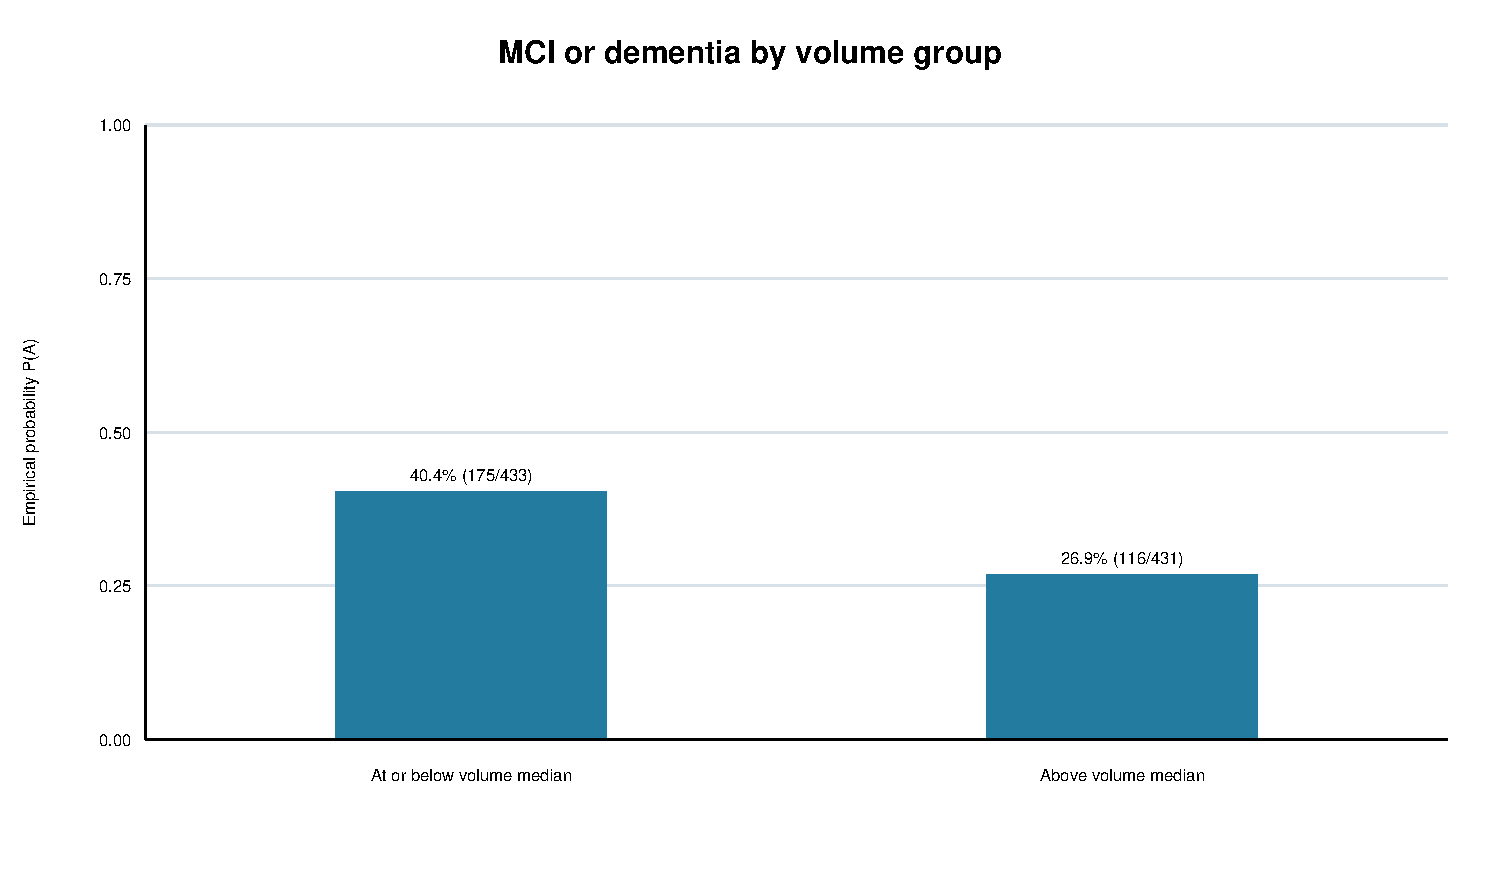
\includegraphics[width=.9\linewidth]{figures/phase2/group_probabilities.pdf}\caption{MCI or dementia probability by median-defined volume group; counts and group denominators shown.}\label{fig:group}\end{figure}
\begin{figure}[H]\centering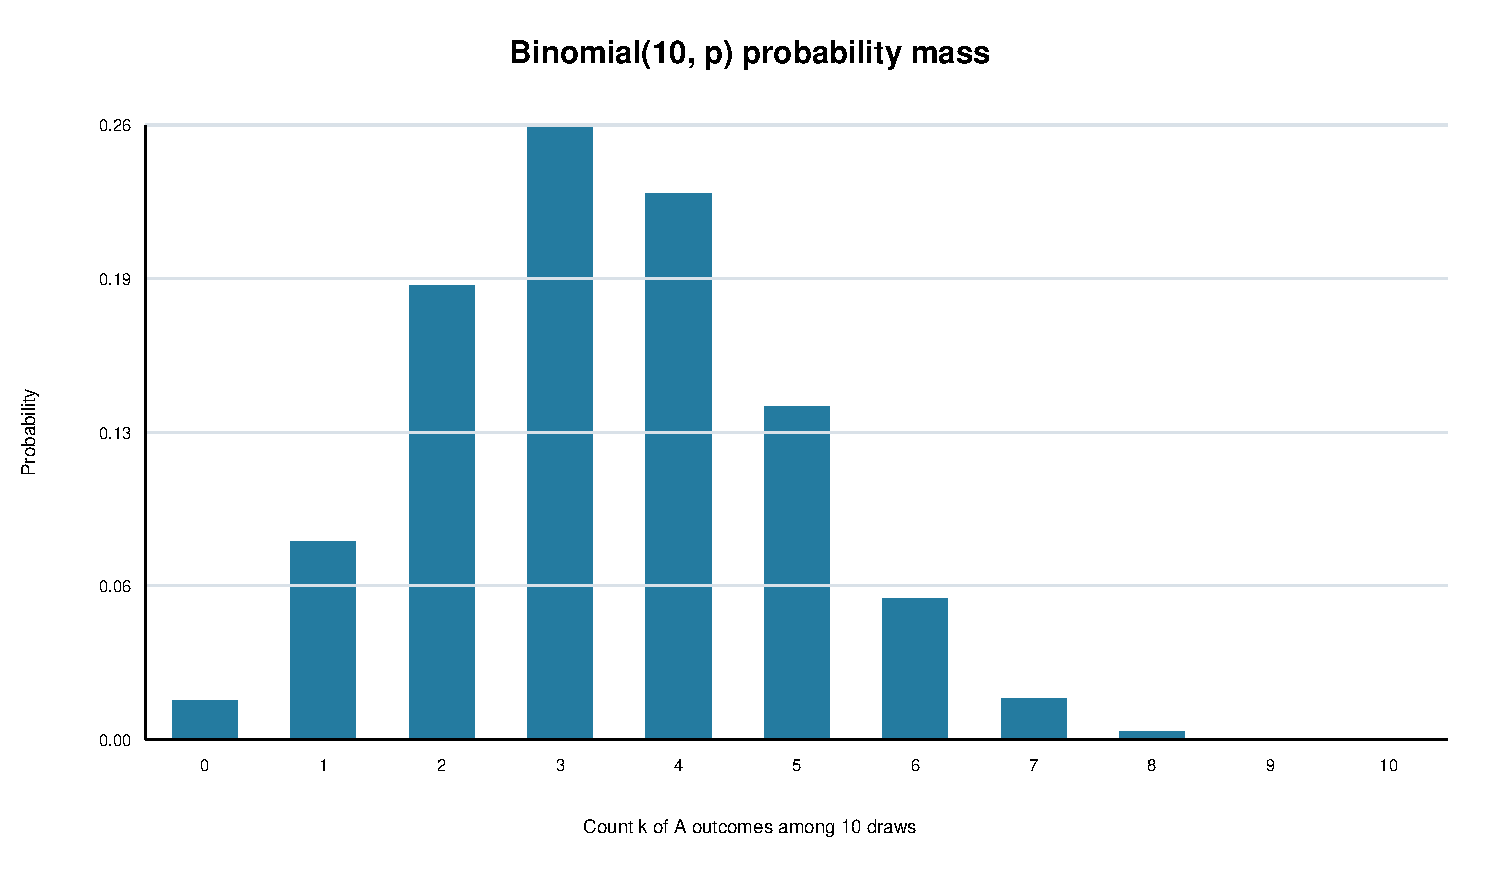
\includegraphics[width=.88\linewidth]{figures/phase2/binomial_pmf.pdf}\caption{Hypothetical $\operatorname{Binomial}(10,p)$ probability mass function.}\label{fig:binom}\end{figure}
\begin{figure}[H]\centering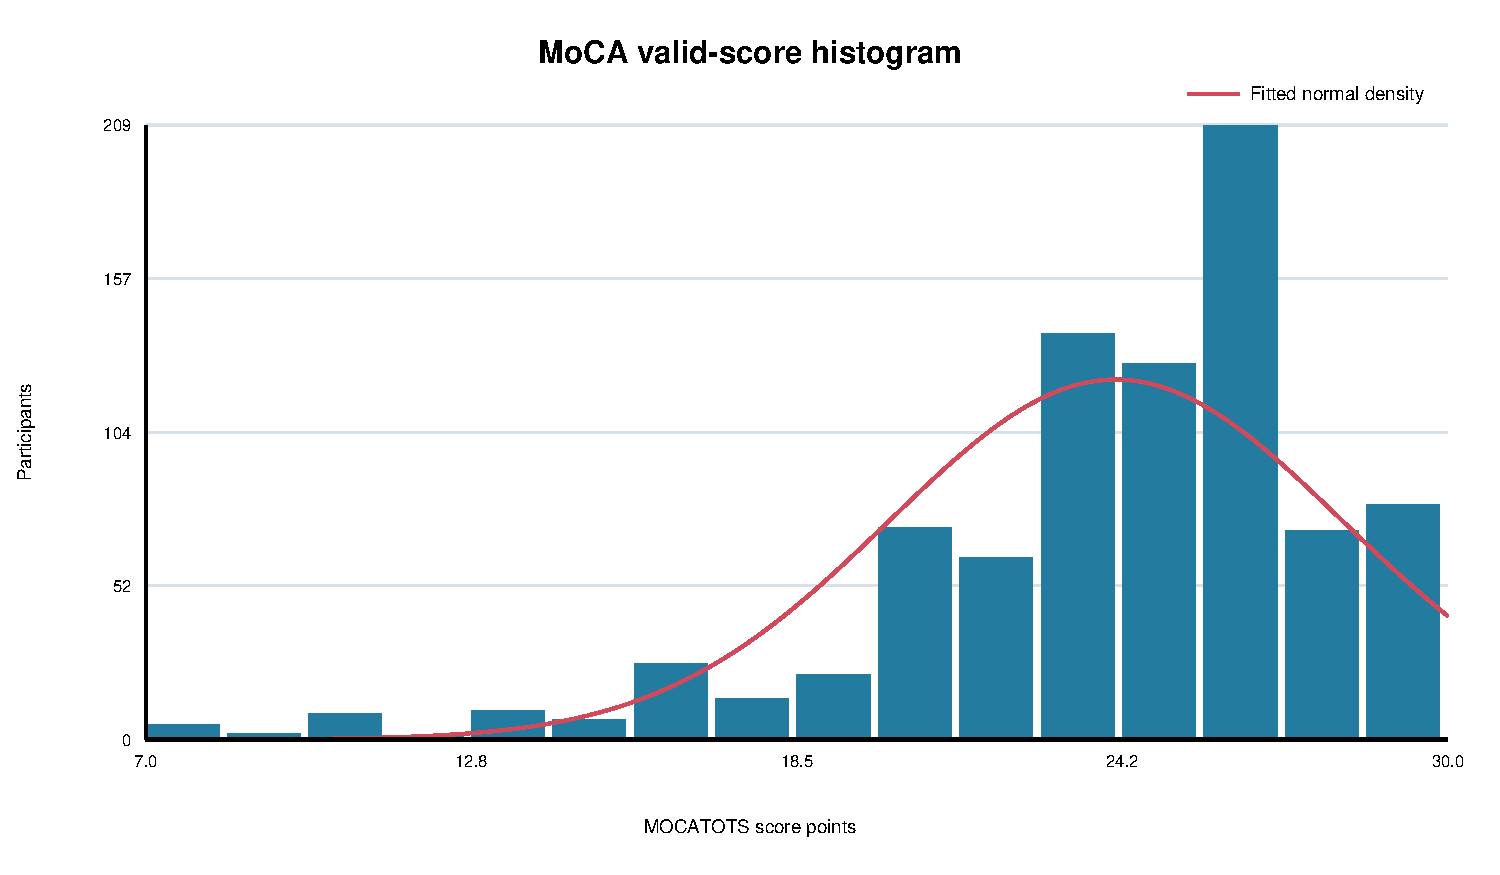
\includegraphics[width=.85\linewidth]{figures/phase2/moca_histogram.pdf}\caption{Valid MOCATOTS histogram and fitted normal density overlay.}\label{fig:moca}\end{figure}
\begin{figure}[H]\centering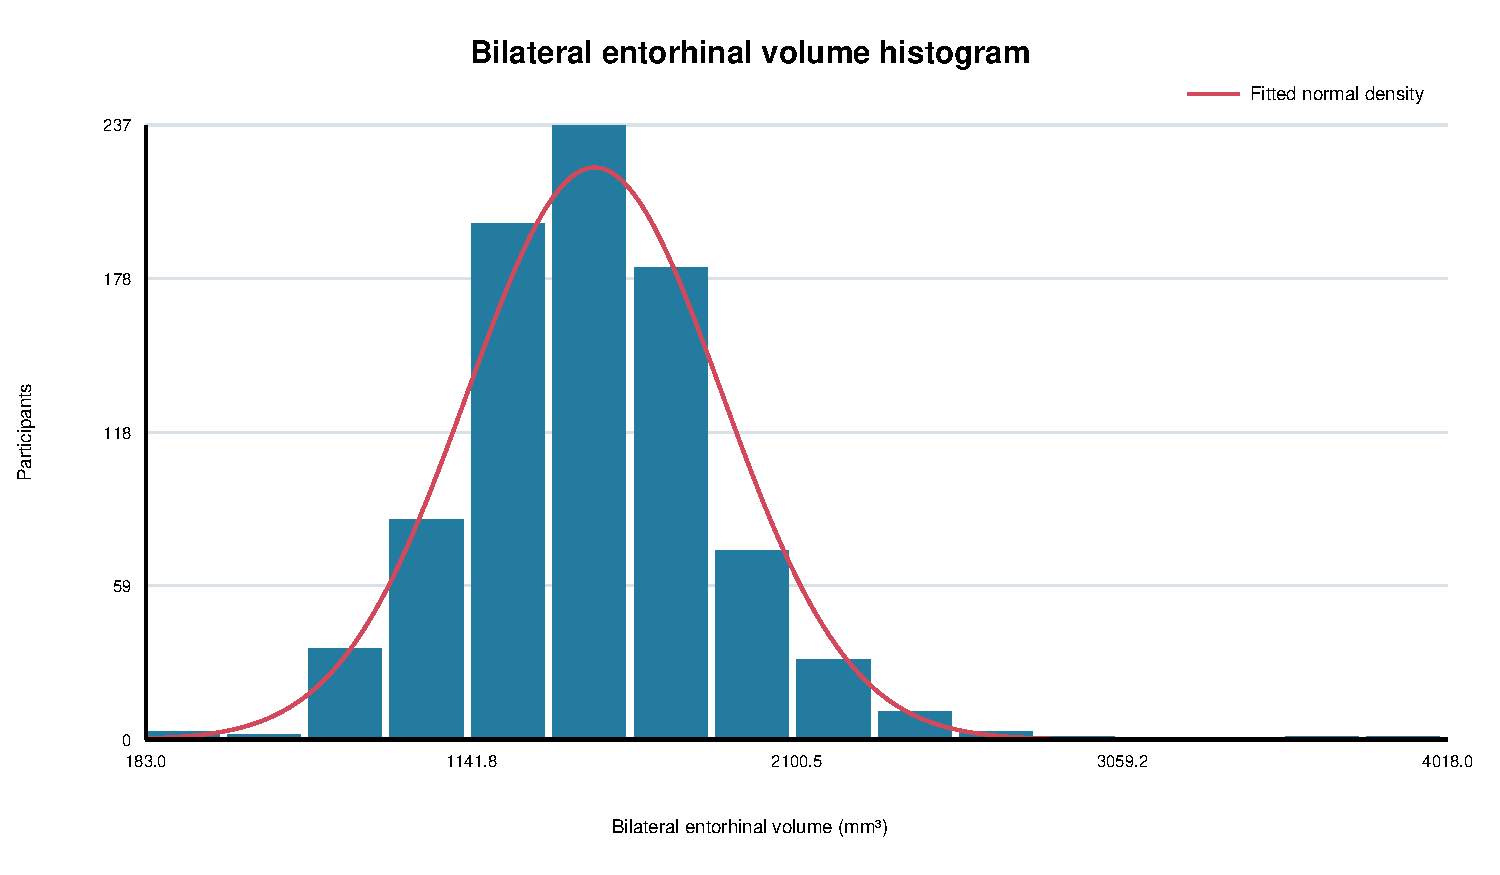
\includegraphics[width=.85\linewidth]{figures/phase2/volume_histogram.pdf}\caption{Valid bilateral volume histogram and fitted normal density overlay.}\end{figure}
\begin{figure}[H]\centering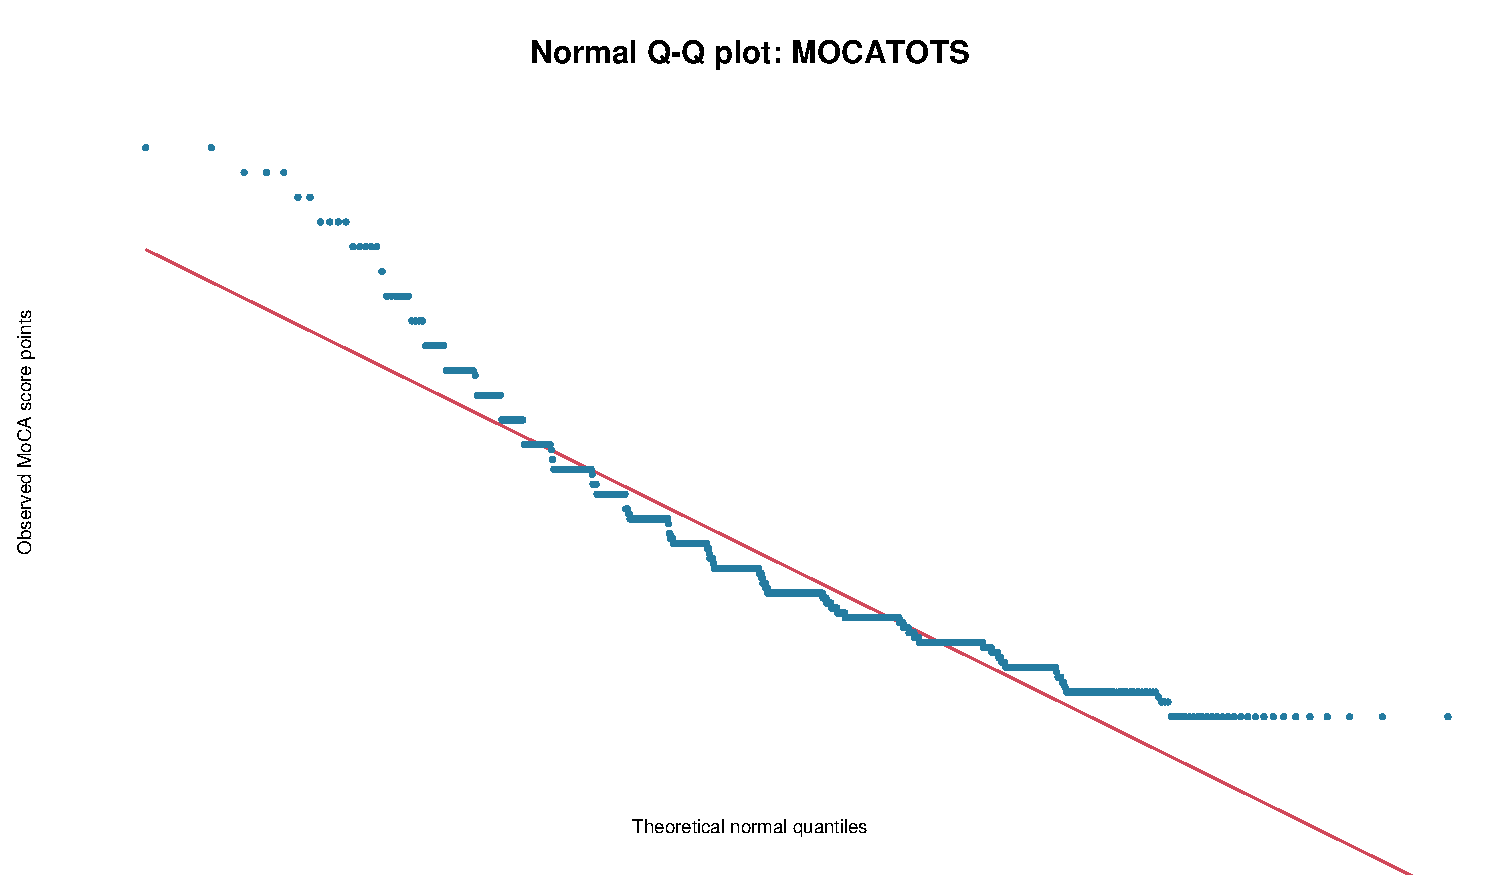
\includegraphics[width=.85\linewidth]{figures/phase2/moca_qq.pdf}\caption{MoCA normal Q--Q plot.}\end{figure}
\begin{figure}[H]\centering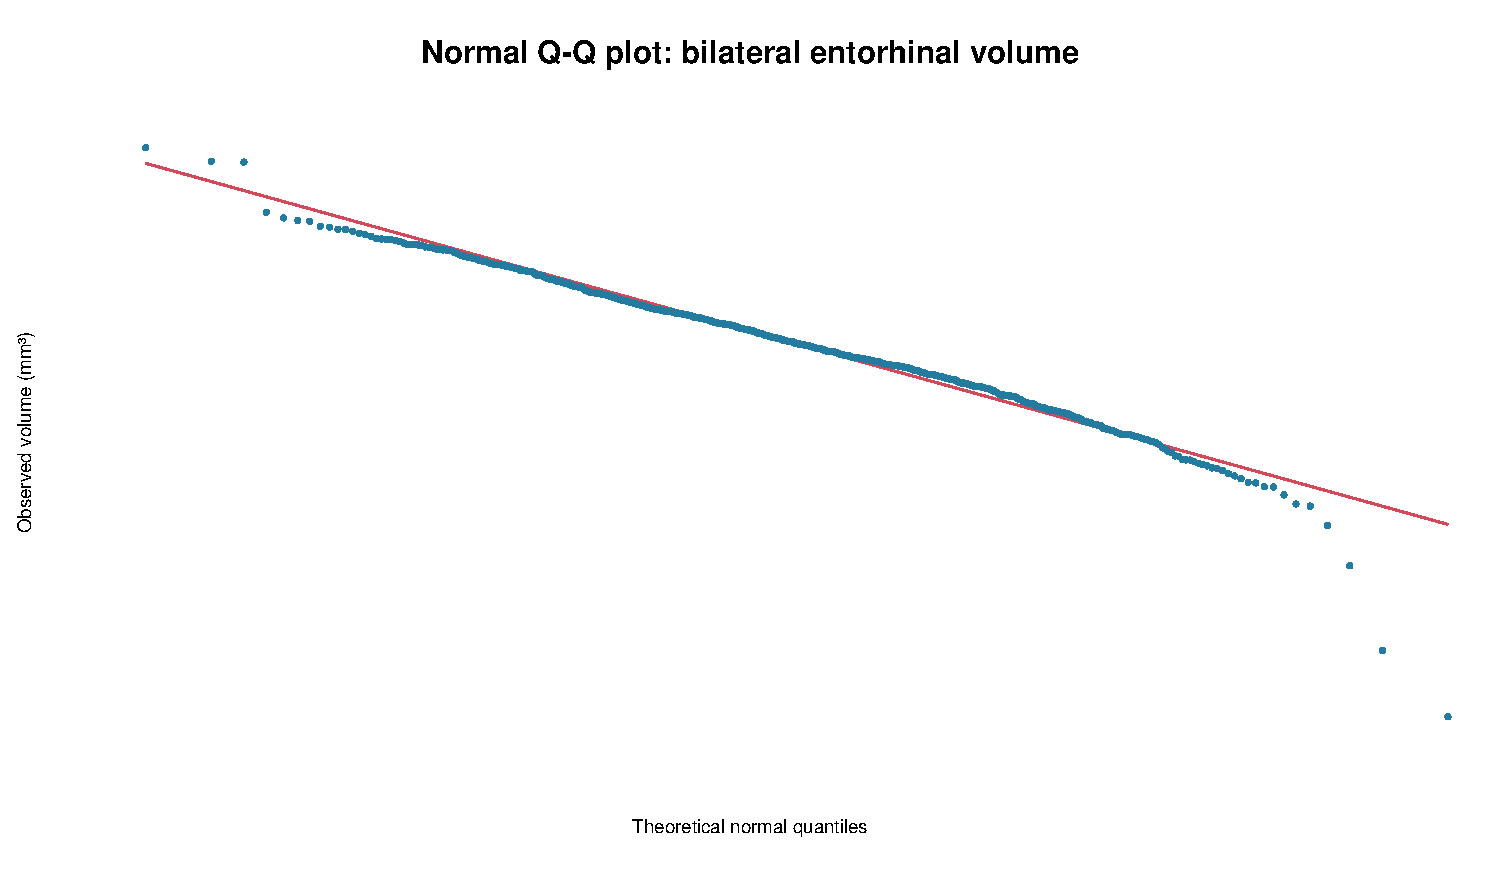
\includegraphics[width=.85\linewidth]{figures/phase2/volume_qq.pdf}\caption{Bilateral volume normal Q--Q plot.}\label{fig:vqq}\end{figure}
\section{MoCA and MRI covariance}
For 856 pairwise-complete age-eligible participants, sample covariance using denominator $n-1$ is 307.5754 score-points$\cdot$mm$^3$, and Pearson correlation is $r=0.2047$. The direction is positive and magnitude describes a modest linear association in this subset. Correlation measures linear association only and does not establish causation. Figure~\ref{fig:scatter} labels both measurements and displays the paired cases.
\begin{figure}[H]\centering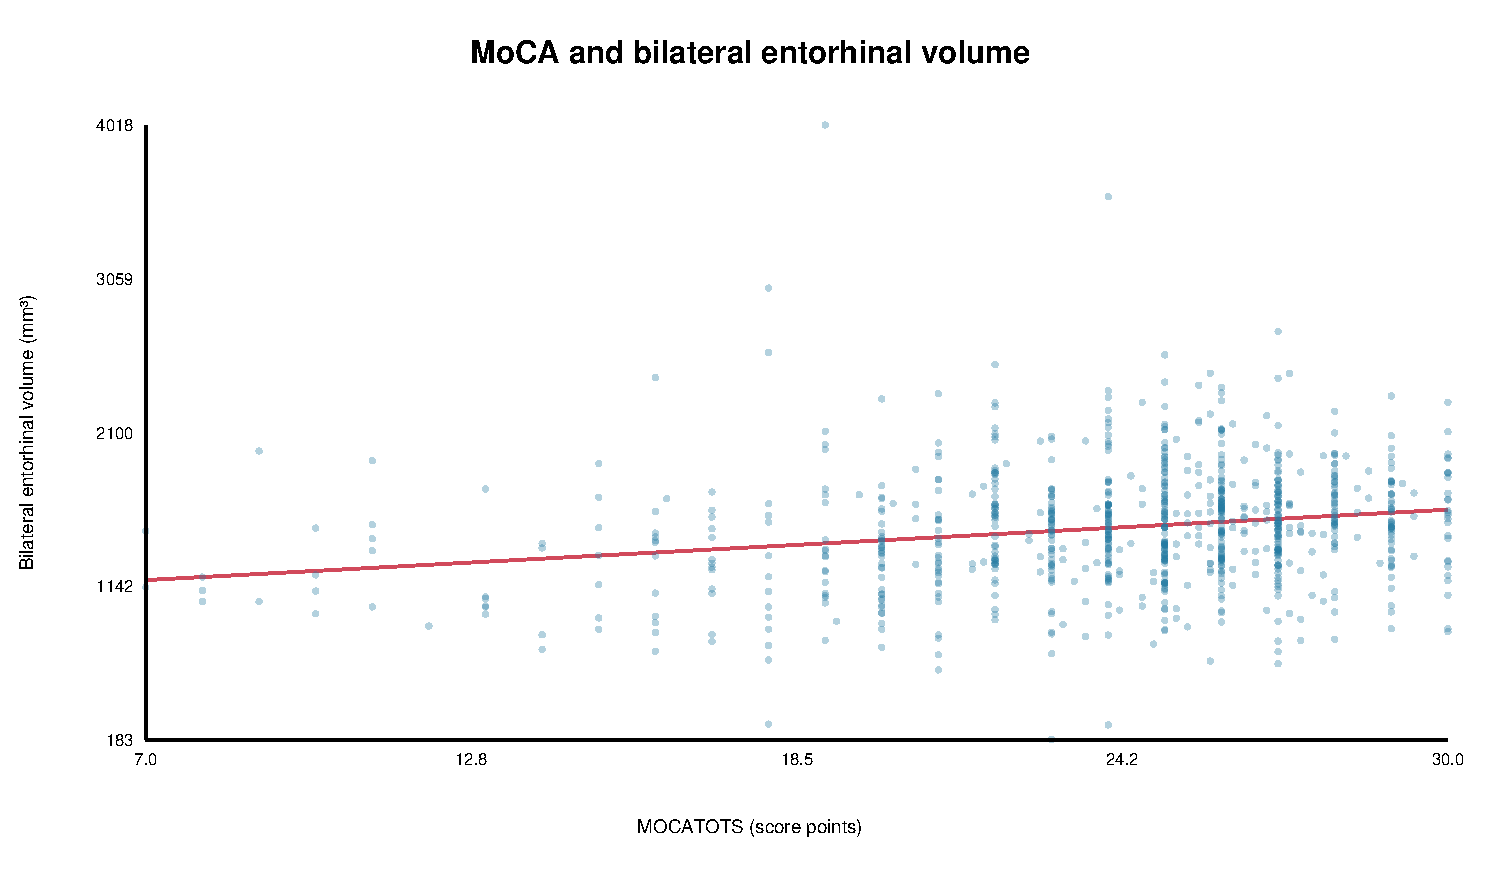
\includegraphics[width=.9\linewidth]{figures/phase2/moca_volume_scatter.pdf}\caption{Pairwise-complete MoCA and bilateral entorhinal volume observations; descriptive fitted line.}\label{fig:scatter}\end{figure}
\section{Bayes' theorem}
From the same table, $P(B\mid A)=n_{11}/n_A=175/291=0.601375$. Bayes' theorem gives $P(A\mid B)P(B)/P(A)=(0.404157)(0.501157)/(0.336806)=0.601375$. The computed sides differ by 0. This updates an event probability within this dataset-defined event system; it is not validated individual diagnostic prediction.
\section{Limitations and conclusion}
This is a descriptive analysis of a supplied clinical/research subset, not a population-representative sample. The files cannot verify baseline status, visit timing, or UDS--MRI contemporaneity. UDS values are processed/imputed; the original missingness mask and imputation method are unavailable. The median split is a descriptive partition, and empirical probabilities are not causal or clinical predictions. Normal plots are visual assessments; no observations were removed under the outlier rule. The data show differing empirical frequencies across volume groups and a positive descriptive linear association between MoCA and volume, subject to these design limits.
\section*{Reproducibility and data definitions}
Run \texttt{python3 src/phase2\_analysis.py} (or the bundled GapGPT Python runtime command documented in README) from the repository root. Results and audit tables are in \texttt{reports/phase2/}, figures in \texttt{figures/phase2/}. The original participant-level CSVs are not copied into generated reports. Phase 1 files remain separate.
\begin{thebibliography}{9}\bibitem{data}National Alzheimer’s Coordinating Center. Prepared course-subset CSVs: \texttt{udslong\_imputed.csv} and \texttt{mriscanclean.csv}. Data dictionary and preprocessing details were not supplied with this repository.\end{thebibliography}
\end{document}
